% Trailing asterisk to suppress section number
\section*{Task 1: SQL injections}

\subsection*{Exercises:}
\begin{enumerate}
\item The input field on the BadStore website in which a SQL injection was performed is that for the email address on the login page, shown in upper half of \autoref{fig:sql1}. The result---being logged on as the administrator---is shown in the lower half of the figure.
\begin{figure}[h!]
	\caption{SQL Injection and Logged in as Administrator}
        \label{fig:sql1}
	\centering 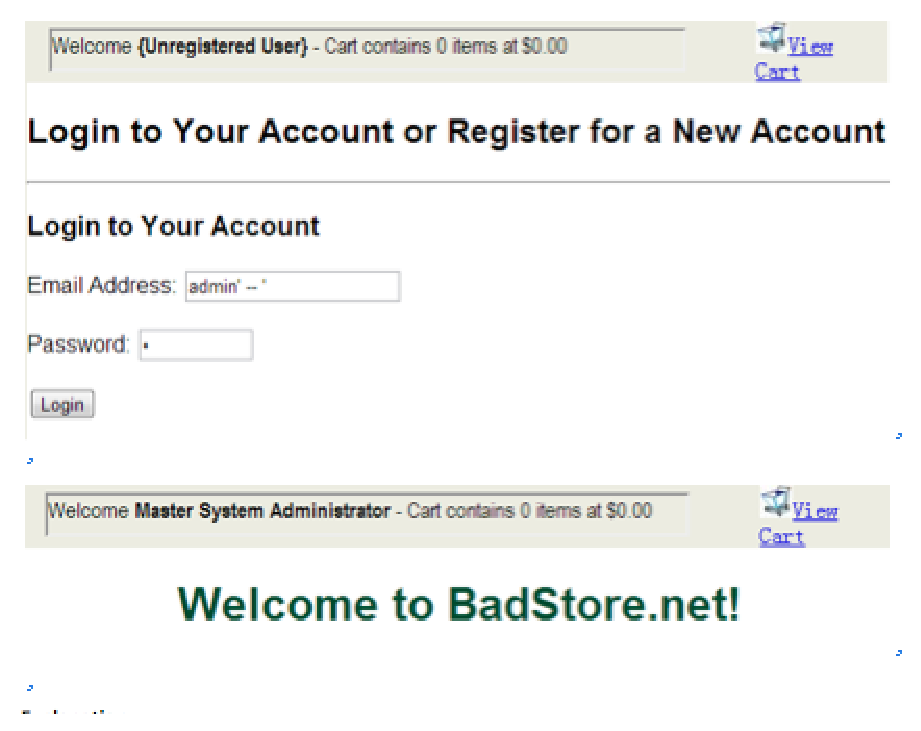
\includegraphics[height=2.5in]{sqli1}
\end{figure}
  
  \textbf{Explanation} Without injection, the SQL code executed when a login request is made is believed to be \lstinline{SELECT * FROM user WHERE EmailAddress = 'emailaddress' AND Password = 'password'}. Then during the injection, we input \lstinline{admin '--'} in the text box for the email address and some arbitrary password in the text box for the password. The WHERE condition is altered into \lstinline{WHERE EmailAddress = 'admin' -- ' AND Password = 'password'}, where the part following the two dashes is interpreted as a SQL comment. In other words, the WHERE condition is turned into \lstinline{WHERE EmailAddress = 'admin'}. Thus there is no need for a password and we can directly log into the admin account.
\item The login page for host \ip{192.168.2.134} and that it was was circumvented successfully using SQL injection is shown in \autoref{fig:sql2}.
\begin{figure}[h!]
	\caption{SQL Injection and the Result}
        \label{fig:sql2}
	\centering 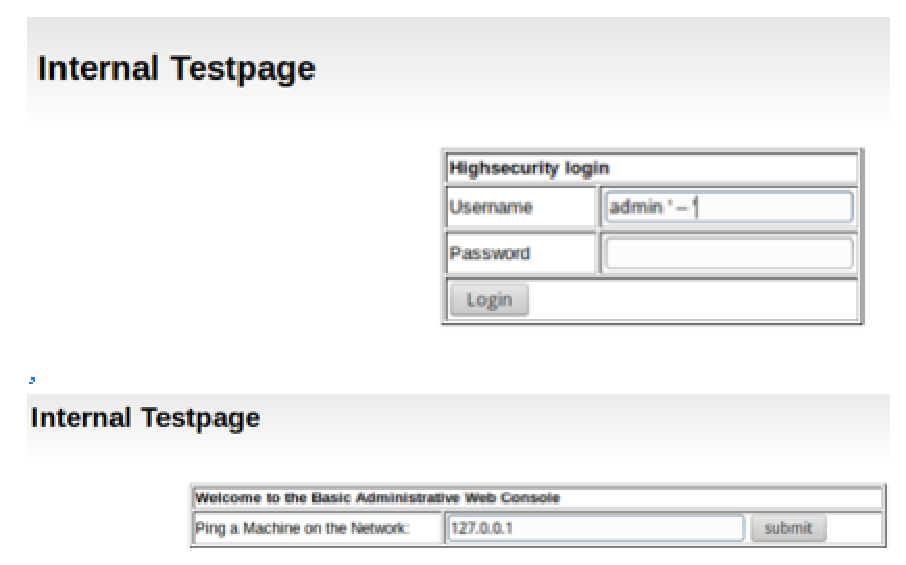
\includegraphics[height=2.5in]{sqli2}
\end{figure}
\\
  \textbf{Explanation} The underlying SQL code for the login screen for host \ip{192.168.2.134} is believed to be the same as before: without injection, the SQL code is thought to be \lstinline{SELECT * FROM user WHERE UserName = 'username' AND Password = 'password'}. Then during the injection, we input \lstinline{admin '--'} in the text box for the username and some arbitrary password in the text box for the password. The WHERE condition is altered into \lstinline{WHERE UserName = 'admin' -- ' AND Password = 'password'} (or equivalently, \lstinline{WHERE UserName = 'admin'}). So there is no need for a password and we can directly log into the admin account.
\item \textbf{Prepared Statement} 
  A prepared statement, which is also called a parametrized statement, is a SQL query with variables inside of it. That is to say, we prepare the query with blank spots to fill and it will automatically protect the query from SQL injection.

  Here is a code snippet for using a prepared statement in PHP\cite{php}:
  \begin{lstlisting}[language = php]
    stmt = dbh->prepare("INSERT INTO REGISTRY (name, value) VALUES (:name, :value)");
    stmt->bindParam(':name', name);
    stmt->bindParam(':value', value);
  \end{lstlisting}

  In our case, a system administrator could prevent the SQL injections of the previous exercises by using a prepared statement such as the following:
  \begin{lstlisting}
    prepare("SELECT * FROM user WHERE UserName = :username AND Password = :password");
    bind(':username', username);
    bind(':password', password);
  \end{lstlisting}
  
  \textbf{Explanation}
  There are two variables in the prepared statement: username and password. Without injection, for instance with the username \lstinline{admin} and the password \lstinline{test}, the SQL query for logging on would be \lstinline{SELECT * FROM user WHERE username = 'admin' AND password = 'test'}. During an injection attempt, for instance with the username \lstinline{admin' --} and password \lstinline{123}, the SQL query becomes \lstinline{SELECT * FROM user WHERE username = 'admin\' --' AND password = '123'}. This is because the binding system will automatically change the input to protect the query. Thus, the SQL injection doesn't work in this situation.
\item The school lost all the student records because the table Students in the database is dropped by SQL injection. The SQL statement intended to be executed can be assumed to be of the form \lstinline{INSERT INTO Students VALUES ('Robert');}. The SQL injection had this query altered into the following two statements and comment: \lstinline{INSERT INTO Students VALUES ('Robert'); DROP TABLE Students; --');}. When the query is executed, the table Students will be dropped.

  What the school should do is to sanitize the database inputs by utilizing prepared statements as mentioned above. They can create the prepared statement as follows:
  \begin{lstlisting}
    prepare("INSERT INTO Students VALUES (':name')");
    bind(':name',name);
  \end{lstlisting}

\end{enumerate}
